\documentclass{article}
\usepackage[linesnumbered,ruled,vlined]{algorithm2e}
\usepackage{amsmath,amsfonts, amsthm, amssymb}
\usepackage{dsfont}
\usepackage{cases}
\usepackage{tablefootnote,graphicx}
\usepackage{natbib}
\usepackage{caption}
\usepackage{longtable}

\bibliographystyle{abbrvnat}
\usepackage{refcount}
\usepackage{geometry}
\usepackage{booktabs}
\usepackage{xcolor,colortbl}
\geometry{verbose,tmargin=1in,bmargin=1in,lmargin=1in,rmargin=1in}
\usepackage{makecell}
\usepackage{multirow}
\usepackage{float}
\usepackage[unicode=true,
 bookmarks=false,
 breaklinks=false,pdfborder={0 0 1},colorlinks=false]
 {hyperref}
\hypersetup{colorlinks,citecolor=blue,filecolor=blue,linkcolor=blue,urlcolor=blue}
\newtheorem{lemma}{Lemma}
\newtheorem{remark}{Remark}
\newtheorem{theorem}{Theorem}
\newtheorem{definition}{Definition}
\newcounter{tmp}

% Title and Author Information
\title{Automotive Clustering}

\author{
    Guo Yu \\
    School of Information Science and Technology\\
    ShanghaiTech University\\
    2022533174
    \texttt{yuguo2022@shanghaitech.edu.cn} \\
    \and  
    Linzheng Tang \\
    School of Information Science and Technology \\
    ShanghaiTech University\\
    2022533087
    \texttt{tanglzh2022@shanghaitech.edu.cn} \\
    \and  
    Guanpeng Long \\
    School of Information Science and Technology \\
    ShanghaiTech University\\ 
    2022533090
    \texttt{longgp2022@shanghaitech.edu.cn} \\
  }

\begin{document}
\maketitle
\begin{abstract}
    This article presents findings from a competition on the TianChi platform
    (\url{https://tianchi.aliyun.com/competition/entrance/531892}), detailing the employed data preprocessing methods,
    dimensionality reduction techniques such as Principal Component Analysis (PCA) and factor analysis, as well as a comparative performance analysis of three representative clustering algorithms.
    Numerical results, visualizations, and practical implications are discussed.
    Recommendations for the most effective solution to the problem are also provided.

\end{abstract}

\section{Introduction}
The objective of this study is to cluster 205 automotive products and identify competitors of Volkswagen brand products using non-parametric algorithms.
The data will undergo preprocessing involving correlation and factor analysis, PCA, and the application of three prominent clustering algorithms: K-means for prototype-based clustering, DBSCAN for density-based clustering, and DIANA for hierarchical clustering.

\section{Data Preprocessing}
\subsection{Premise}

\paragraph{Definition}
A critical aspect of this analysis is the definition of a competitor.
Based on general automotive market standards, two car models are considered competitors if their price and car type are sufficiently similar.
Thus, two key features—``carbody'' and ``price''—are prioritized during the clustering process.

Consequently, the final results will filter out competitors in each cluster based on their prices, which must fall within a specific range around the mean price of the Volkswagen cluster.

\paragraph{Feature Selection}
In the automotive market, the car brand significantly influences consumer decisions.
Therefore, the ``CarName'' feature was parsed to extract a new feature labeled ``brand'' for clustering purposes.
The feature ``car\_ID'' was deemed irrelevant to the clustering process and subsequently removed.

\subsection{Data Cleaning}

\paragraph{Spelling Errors and Abbreviations}
Instances of spelling errors and abbreviations were identified within the ``brand'' feature.
Specifically, entries with ``car\_ID'' 190 and 191 abbreviated ``Volkswagen'' as ``vw'', while entry with ``car\_ID'' 183 misspelled ``Volkswagen'' as ``vokswagen''.
These discrepancies were rectified using a pandas DataFrame.

\paragraph{Z-score Analysis}
The Z-score, which indicates the deviation of a data point from the mean, is calculated using the formula:
\begin{equation}
    Z = \frac{X - \mu}{\sigma}
\end{equation}
where \( X \) represents the data point, \( \mu \) is the dataset mean, and \( \sigma \) is the standard deviation.

This formula was applied to numerical features with a threshold set at 3.0.
Any data point with an absolute Z-score exceeding 3.0 was classified as an outlier.
The analysis identified 24 outliers; however, further research indicated their validity.
For instance, a compression ratio exceeding 20 is typical for diesel engines.
Thus, all 24 outliers were retained in the dataset.

\section{Hierarchical Clustering}
The methodology integrates factor analysis \cite{Gorsuch1983}, a dimensionality reduction technique, with DIANA hierarchical clustering.
This combined approach serves as the primary method, which will be compared with the other two basic methods in subsequent sections.

\subsection{Pre-processing for Factor Analysis}
Prior to applying factor analysis, the Kaiser–Meyer–Olkin (KMO) test and Bartlett's sphericity test were conducted to assess the data's suitability for factor analysis.
The resulting KMO score of 0.8035, exceeding the 0.7 threshold, indicates a satisfactory level of sample adequacy.
Additionally, Bartlett's p-value of 0.0, below the 0.05 threshold, signifies that the variables are sufficiently correlated for factor analysis.

Given the significance of the features ``price'' and ``carbody'', these variables were not subjected to feature compression.

\subsection{Variance Analysis}
The principal factor analysis was conducted using 14 factors, accounting for 96.46\% of the variance without rotation.

\begin{table}[H]
    \centering
    \caption{Factor Analysis Results}
    \small
    \begin{tabular}{cccc}
        \toprule
        \textbf{Index} & \textbf{Eigenvalue} & \textbf{Variance Contribution Rate} & \textbf{Cumulative Variance Contribution Rate} \\
        \midrule
        0              & 6.602030            & 0.330101                            & 0.330101                                       \\
        1              & 2.942172            & 0.147109                            & 0.477210                                       \\
        2              & 2.732131            & 0.136607                            & 0.613817                                       \\
        3              & 1.441222            & 0.072061                            & 0.685878                                       \\
        4              & 1.083674            & 0.054184                            & 0.740061                                       \\
        5              & 0.908388            & 0.045419                            & 0.785481                                       \\
        6              & 0.721047            & 0.036052                            & 0.821533                                       \\
        \bottomrule
    \end{tabular}
\end{table}

The first seven factors account for over 80\% of the variance, which is conventionally accepted as the number of factors to retain.

\subsection{Orthogonal Rotation}
\paragraph{Quartimax Rotation} Upon reapplying the analysis, it was observed that certain factors exhibited closely related influences on specific features, such as factors 6 and 7 for ``carwidth'' and factors 4 and 5 for ``carheight''.

\begin{table}[H]
    \centering
    \caption{Factor Loadings Before Rotation}
    \begin{tabular}{lccccccc}
        \toprule
                  & \textbf{Factor 1} & \textbf{Factor 2} & \textbf{Factor 3} & \textbf{Factor 4} & \textbf{Factor 5} & \textbf{Factor 6} & \textbf{Factor 7} \\
        \midrule
        carwidth  & 0.879082          & -0.145625         & 0.131856          & 0.083021          & 0.106253          & 0.051310          & 0.046592          \\
        carheight & 0.248923          & -0.356886         & 0.561215          & -0.459978         & 0.038325          & 0.037018          & 0.232987          \\
        \bottomrule
    \end{tabular}
\end{table}

After removing features with high correlation, the resulting factors were considered orthogonal, and the ``quartimax'' rotation method was applied to minimize the number of factors required to explain each variable, yielding the final factor results.

\paragraph{ANOVA}
An analysis of variance (ANOVA) was conducted, yielding the following results:
\begin{table}[H]
    \centering
    \caption{ANOVA Results}
    \begin{tabular}{lcccccl}
        \toprule
        \textbf{Source} & \textbf{df} & \textbf{Sum of Squares}  & \textbf{Mean Square}     & \textbf{F} & \textbf{p-value}           & \textbf{Variable} \\
        \midrule
        C(type)         & 3.0         & $9.170561 \times 10^{9}$ & $3.056854 \times 10^{9}$ & 159.63     & $6.181610 \times 10^{-53}$ & price             \\
        Residual        & 201.0       & $3.849078 \times 10^{9}$ & $1.914964 \times 10^{7}$ & --         & --                         & price             \\
        C(type)         & 3.0         & $8.154253 \times 10^{8}$ & $2.718084 \times 10^{8}$ & 24.49      & $1.508741 \times 10^{-13}$ & carbody           \\
        Residual        & 201.0       & $2.231129 \times 10^{9}$ & $1.110014 \times 10^{7}$ & --         & --                         & carbody           \\
        C(type)         & 3.0         & $5.996481 \times 10^{2}$ & $1.998827 \times 10^{2}$ & 180.95     & $7.488293 \times 10^{-57}$ & factor\_type      \\
        Residual        & 201.0       & $2.220299 \times 10^{2}$ & $1.104627 \times 10^{0}$ & --         & --                         & factor\_type      \\
        \bottomrule
    \end{tabular}
\end{table}
The p-value below 0.05 indicates the rejection of the null hypothesis, confirming significant differences between factor means.

\subsection{DIANA}
Following the acquisition of the resulting factors, normalization was performed using a standard scaler, incorporating the features ``price'' and ``carbody''.
The resulting dendrogram is presented below:
\begin{figure}[H]
    \centering
    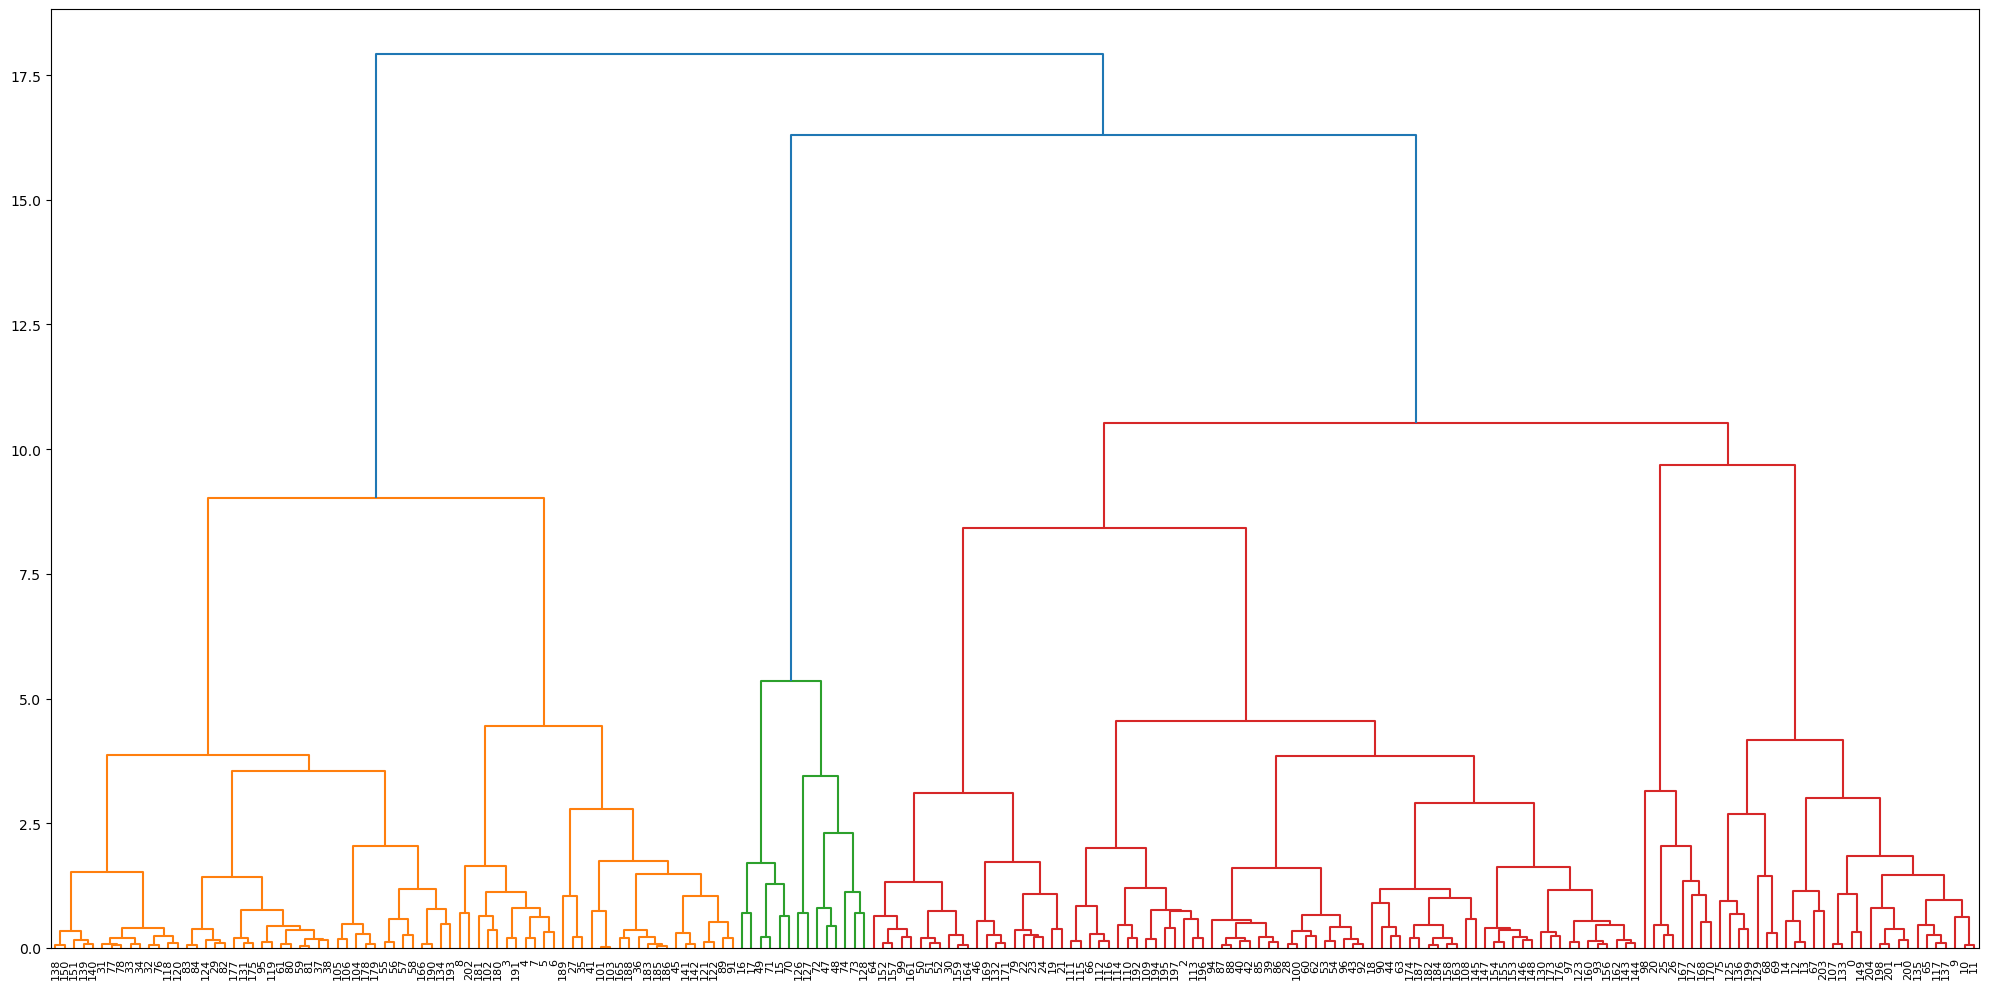
\includegraphics[width=0.6\textwidth]{image/paper/link_tree.png}
    \caption{Hierarchy Dendrogram}
    \label{tree}
\end{figure}
A noticeable leap in the middle blue line from scale 16 to 5.5 suggests that the tree should be cut at scale 10, resulting in four clusters.
Subsequently, product portraits were created based on price and other factors:

\begin{table}[H]
    \centering
    \caption{Carbody Proportion by Type}
    \small
    \begin{tabular}{llccccc}
        \toprule
        \textbf{ID} & \textbf{Type}                 & \textbf{Convertible(\%)} & \textbf{Hardtop(\%)} & \textbf{Hatchback(\%)} & \textbf{Sedan(\%)} & \textbf{Wagon(\%)} \\
        \midrule
        0           & Mid-high end comfortable cars & 8.33                     & 13.89                & 13.89                  & 55.56              & 8.33               \\
        1           & Mid price comfortable cars    & 0.00                     & 0.00                 & 28.05                  & 51.22              & 20.73              \\
        2           & Mid price practical cars      & 1.37                     & 0.00                 & 57.53                  & 34.25              & 6.85               \\
        3           & Luxury Premium Cars           & 14.29                    & 21.43                & 0.00                   & 64.29              & 0.00               \\
        \bottomrule
    \end{tabular}
\end{table}

\begin{table}[H]
    \centering
    \caption{Mean Price by Type}
    \begin{tabular}{lll}
        \toprule
        \textbf{ID} & \textbf{Type}                 & \textbf{Mean Price (\$)} \\
        \midrule
        0           & Mid-high end comfortable cars & 17,184.9                 \\
        1           & Mid price comfortable cars    & 9,745.8                  \\
        2           & Mid price practical cars      & 10,964.1                 \\
        3           & Luxury Premium Cars           & 35,967.1                 \\
        \bottomrule
    \end{tabular}
\end{table}

\subsection{Related Clusters}
Upon clustering, Volkswagen products were identified within the categories of Mid Price Comfortable Cars and Mid Price Practical Cars.
The overview of cluster information is presented below:
\begin{table}[H]
    \centering
    \caption{Volkswagen Product Distribution}
    \begin{tabular}{lll}
        \toprule
        \textbf{Cluster}           & \textbf{Product Number} & \textbf{Mean Price (\$)} \\
        \midrule
        Mid price comfortable cars & 4                       & 9,777.5                  \\
        Mid price practical cars   & 8                       & 10,227.5                 \\
        \bottomrule
    \end{tabular}
\end{table}
\begin{table}[H]
    \centering
    \small
    \caption{Related Car-Type Proportion and Mean Price}
    \begin{tabular}{llllll}
        \toprule
        \textbf{Type}              & \textbf{Mean Price (\$)} & \textbf{Sedan(\%)} & \textbf{Hatchback(\%)} & \textbf{Wagon(\%)} & \textbf{Convertible(\%)} \\
        \midrule
        Volkswagen Comfortable     & 9,777.5                  & 100.0              & 0.0                    & 0.0                & 0.0                      \\
        Volkswagen Practical       & 10,227.5                 & 62.5               & 12.5                   & 12.5               & 0.0                      \\
        Mid Price Comfortable Cars & 9,745.8                  & 51.2               & 28.0                   & 20.73              & 0.0                      \\
        Mid Price Practical Cars   & 10,964.0                 & 34.25              & 57.53                  & 6.85               & 1.37                     \\
        \bottomrule
    \end{tabular}
\end{table}

\section{Prototype Clustering}
K-means \cite{MacQueen1967} was selected as the representative method for prototype clustering.
This section outlines the entire clustering process.

\subsection{PCA and Hyper-parameters}
\paragraph{PCA}
The data was first scaled using a standard scaler, with an additional weight of 1.25 applied to the features ``price'' and ``carbody'' due to their significance.
PCA was then performed on the scaled dataset, with the dimension set to 7 to capture 80\% of the variance.

\paragraph{Hyper-parameters}
The number of clusters was determined using the Elbow Plot:
\begin{figure}[H]
    \centering
    \begin{minipage}{0.3\textwidth}
        \centering
        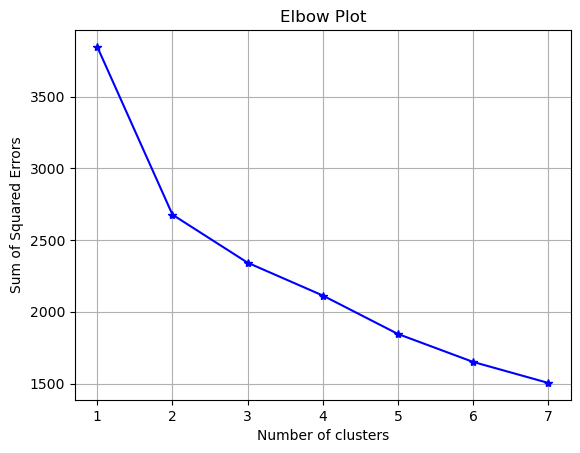
\includegraphics[width=\textwidth]{image/paper/elbow.png}
        \caption{Elbow Plot}
        \label{elbow}
    \end{minipage}\hfill
    \begin{minipage}{0.6\textwidth}
        \small
        Despite the plot indicating a clear inflection point at \( k=2 \), for practical considerations and to achieve lower SSE, \( k=5 \) was chosen, utilizing the ``k-means++'' initialization method for rapid convergence.
    \end{minipage}
\end{figure}

\subsection{K-means}
The hyper-parameters were applied to K-means clustering, resulting in product portraits similar to those in the previous section:
\begin{table}[H]
    \small
    \caption{Carbody Proportion by Type}
    \begin{tabular}{llccccc}
        \toprule
        \textbf{ID} & \textbf{Type}              & \textbf{Convertible(\%)} & \textbf{Hardtop(\%)} & \textbf{Hatchback(\%)} & \textbf{Sedan(\%)} & \textbf{Wagon(\%)} \\
        \midrule
        0           & Mid price practical cars   & 1.02                     & 1.02                 & 37.76                  & 47.96              & 12.24              \\
        1           & Mid price comfortable cars & 4.23                     & 5.63                 & 36.62                  & 39.44              & 14.08              \\
        2           & Luxury Premium Cars        & 15.38                    & 15.38                & 7.69                   & 61.54              & 0.00               \\
        3           & Low price economical cars  & 0.00                     & 0.00                 & 66.67                  & 33.33              & 0.00               \\
        4           & High-end commercial cars   & 0.00                     & 7.14                 & 0.00                   & 71.43              & 21.43              \\
        \bottomrule
    \end{tabular}
\end{table}



The resulting PCA cluster visualization of the first three principal components is displayed below:


\begin{figure}[H]
    \centering
    \begin{minipage}{0.5\textwidth}
        \centering
        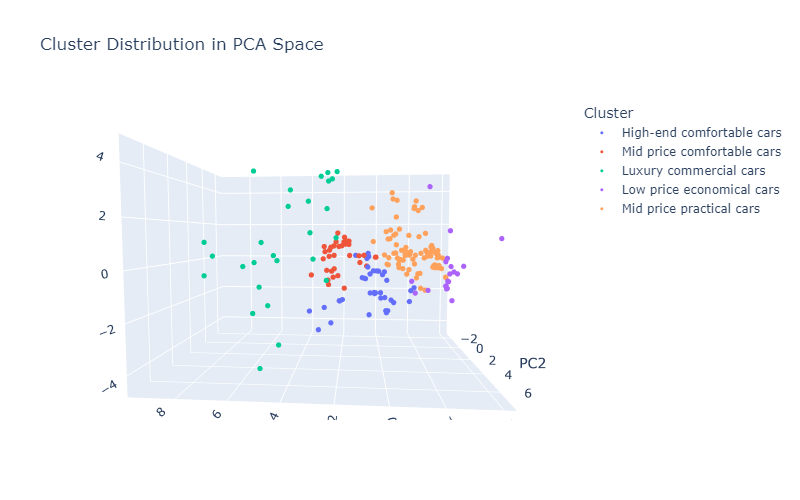
\includegraphics[width=1\textwidth]{image/paper/kmeans.png}
        \caption{PCA Visualization}
        \label{pca1}
    \end{minipage}\hfill
    \begin{minipage}{0.5\textwidth}
        \begin{table}[H]
            \centering
            \small
            \caption{Mean Price by Type}
            \begin{tabular}{lll}
                \toprule
                \textbf{ID} & \textbf{Type}              & \textbf{Mean Price (\$)} \\
                \midrule
                0           & Mid price practical cars   & 8,214.16                 \\
                1           & Mid price comfortable cars & 15,316.26                \\
                2           & Luxury Premium Cars        & 36,216.27                \\
                3           & Low price economical cars  & 6,495.22                 \\
                4           & High-end commercial cars   & 21,429.64                \\
                \bottomrule
            \end{tabular}
        \end{table}
    \end{minipage}
\end{figure}

\subsection{Related Clusters}
Information pertaining to Volkswagen-related clusters is presented below:
\begin{table}[H]
    \centering
    \caption{Volkswagen Product Distribution}
    \begin{tabular}{lll}
        \toprule
        \textbf{Cluster}           & \textbf{Product Number} & \textbf{Mean Price (\$)} \\
        \midrule
        Mid price practical cars   & 1                       & 9,980.0                  \\
        High-end comfortable cars  & 1                       & 13,295.0                 \\
        Mid price comfortable cars & 10                      & 9,765.5                  \\
        \bottomrule
    \end{tabular}
\end{table}

\begin{table}[H]
    \centering
    \small
    \caption{Related Car-Type Proportion and Mean Price}
    \begin{tabular}{llcccc}
        \toprule
        \textbf{Type}              & \textbf{Mean Price (\$)} & \textbf{Sedan(\%)} & \textbf{Hatchback(\%)} & \textbf{Wagon(\%)} & \textbf{Convertible(\%)} \\
        \midrule
        Volkswagen Comfortable     & 9,765.5                  & 100.00             & 0.00                   & 0.00               & 0.00                     \\
        Volkswagen Practical       & 9,980.0                  & 80.00              & 0.00                   & 10.00              & 10.00                    \\
        Volkswagen High-end        & 13,295.0                 & 0.00               & 100.00                 & 0.00               & 0.00                     \\
        Mid Price Comfortable Cars & 16,190.09                & 62.96              & 7.41                   & 11.11              & 7.41                     \\
        Mid Price Practical Cars   & 8,490.76                 & 25.00              & 75.00                  & 0.00               & 0.00                     \\
        High-end Comfortable Cars  & 14,088.68                & 67.65              & 5.88                   & 26.47              & 0.00                     \\
        \bottomrule
    \end{tabular}
\end{table}

\section{Density Clustering}
DBSCAN \cite{Ester1996} was selected as the representative method for density clustering.
This section outlines the entire clustering process.

\subsection{PCA and Hyper-parameters}
\paragraph{PCA} Similar to the previous section, the data was first scaled using a standard scaler, followed by PCA with a dimension of 7 to capture 80\% of the variance.
The features ``price'' and ``carbody'' received a weight of 1.25 due to their significance.

\paragraph{Hyper-parameters}
Hyper-parameters ``eps'' and ``min\_samples'' were optimized through loop tuning, with the silhouette score serving as the evaluation metric.
The optimal combination of hyper-parameters was determined to be (4.05, 3).

\subsection{DBSCAN}
The hyper-parameters were applied to DBSCAN clustering, resulting in product portraits similar to those in previous sections:
\begin{table}[H]
    \centering
    \small
    \caption{Carbody Proportion by Type}
    \begin{tabular}{llccccc}
        \toprule
        \textbf{ID} & \textbf{Type}       & \textbf{Convertible (\%)} & \textbf{Hardtop (\%)} & \textbf{Hatchback (\%)} & \textbf{Sedan (\%)} & \textbf{Wagon (\%)} \\
        \midrule
        0           & Mid price MPVs      & 2.48                      & 2.97                  & 34.65                   & 47.52               & 12.38               \\
        1           & Luxury premium cars & 33.33                     & 66.67                 & 0.00                    & 0.00                & 0.00                \\
        \bottomrule
    \end{tabular}
\end{table}

\begin{table}[H]
    \centering
    \caption{Mean Price by Type}
    \begin{tabular}{lll}
        \toprule
        \textbf{ID} & \textbf{Type}       & \textbf{Mean Price (\$)} \\
        \midrule
        0           & Mid price MPVs      & 12,961.10                \\
        1           & Luxury premium cars & 34,528.00                \\
        \bottomrule
    \end{tabular}
\end{table}

The resulting PCA cluster visualization of the first three principal components is displayed below:

\begin{figure}[H]
    \centering
    \begin{minipage}{0.5\textwidth}
        \centering
        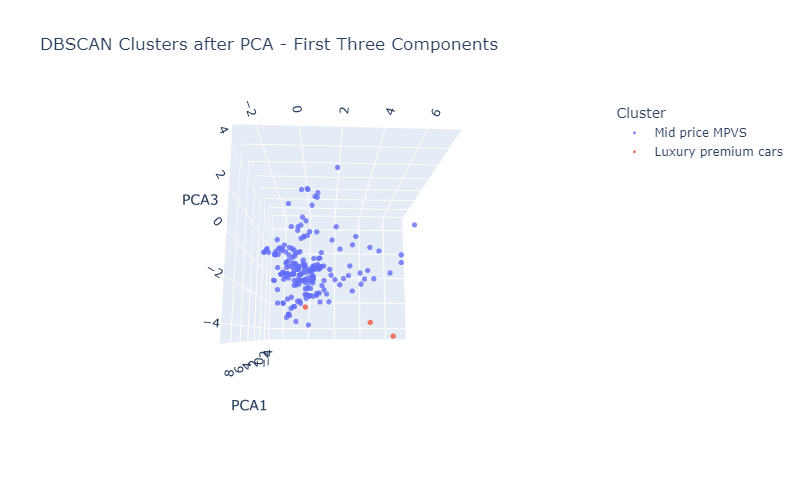
\includegraphics[width=1\textwidth]{image/paper/dbscan.png}
        \caption{PCA Visualization}
        \label{pca2}
    \end{minipage}\hfill
    \begin{minipage}{0.5\textwidth}
        \begin{table}[H]
            \centering
            \caption{Mean Price by Type}
            \begin{tabular}{lll}
                \toprule
                \textbf{ID} & \textbf{Type}       & \textbf{Mean Price (\$)} \\
                \midrule
                0           & Mid price MPVs      & 12,961.10                \\
                1           & Luxury premium cars & 34,528.00                \\
                \bottomrule
            \end{tabular}
        \end{table}

    \end{minipage}
\end{figure}

\subsection{Related Clusters}
Information regarding Volkswagen-related clusters is presented below:

\begin{table}[H]
    \centering
    \caption{Volkswagen Product Distribution}
    \begin{tabular}{lll}
        \toprule
        \textbf{Cluster} & \textbf{Product Number} & \textbf{Mean Price (\$)} \\
        \midrule
        Mid price MPVs   & 12                      & 10,077.5                 \\
        \bottomrule
    \end{tabular}
\end{table}

\begin{table}[H]
    \centering
    \small
    \caption{Related Car-Type Proportion and Mean Price}
    \begin{tabular}{llcccc}
        \toprule
        \textbf{Type}  & \textbf{Mean Price (\$)} & \textbf{Sedan (\%)} & \textbf{Hatchback (\%)} & \textbf{Wagon (\%)} & \textbf{Convertible (\%)} \\
        \midrule
        Volkswagen MPV & 10,077.5                 & 75.00               & 8.33                    & 8.33                & 8.33                      \\
        Mid Price MPVs & 12,961.10                & 47.52               & 34.65                   & 12.38               & 2.48                      \\
        \bottomrule
    \end{tabular}
\end{table}

\section{Result Interpretation and Conclusions}

\subsection{Numerical Results}

\paragraph{Overview}
Given that the competition did not provide definitive answers or evaluation metrics, numerical results from the three clustering algorithms are presented, employing the following common clustering metrics:
\begin{table}[H]
    \centering
    \caption{Clustering Method Evaluation Metrics}
    \label{tab:clustering_scores}
    \begin{tabular}{lccc}
        \toprule
        \textbf{Method}         & \textbf{Silhouette Score} & \textbf{Calinski-Harabasz Score} & \textbf{Davies-Bouldin Score} \\
        \midrule
        Hierarchical Clustering & 0.2835                    & 87.8302                          & 1.2783                        \\
        K-Means                 & 0.1642                    & 36.0311                          & 1.8688                        \\
        DBSCAN                  & 0.3590                    & 9.0123                           & 0.9466                        \\
        \bottomrule
    \end{tabular}
\end{table}

Due to report length constraints, detailed formulas for the aforementioned scores are omitted.

\subsection{Comparison}
\paragraph{DBSCAN}
The DBSCAN algorithm exhibited superior performance in terms of the Davies-Bouldin and silhouette scores, indicating optimal cluster separation and minimal overlap.
However, the algorithm resulted in only two clusters with significant quantity disparities.
Coupled with a notably lower Calinski-Harabasz score, this suggests that the density of data points is neither uniform nor compact, rendering the outcome impractical.

\paragraph{K-means}
K-means demonstrated the least efficiency among the numerical results, with relatively low silhouette and Calinski-Harabasz scores, indicating challenges in cluster separation.
The high Davies-Bouldin score suggests considerable overlap or similarities between clusters.
PCA visualizations revealed that the clusters are relatively compact but exhibit unclear boundaries, particularly for the ``Luxury Premium Cars'' cluster, characterized by a loose structure.
Thus, K-means is deemed more practical than DBSCAN, yet still inefficient.

\paragraph{Factor Analysis and Hierarchical Clustering}
The combined approach significantly outperformed the other two methods in terms of the Calinski-Harabasz score, indicating well-separated and distinct clusters.
A silhouette score approaching 0.3, while not exceptionally high, suggests reasonable cluster definition.
Although a Davies-Bouldin score exceeding 1.0 indicates some overlap, it remains within an acceptable range.
Consequently, this method is considered more practical than both DBSCAN and K-means.

\paragraph{Conclusions}
Taking into account both numerical results and practical considerations, the Factor Analysis and Hierarchical Clustering algorithm is recommended as the final solution to the problem.
Detailed competitor filtering methodologies will be discussed further.

\subsection{Final Result}
Recognizing price as the most significant feature for competing products, specific competitors were identified by filtering Volkswagen-related groups according to a price range of (0.8, 1.2) times the mean price of Volkswagen products in each cluster.

\begin{longtable}{llccccl}
    \caption{Volkswagen Competitors}                                                                                \\
    \toprule
    \textbf{CarName}         & \textbf{Price (\$)} & \textbf{Carbody} & \textbf{Brand} & \textbf{Type}              \\
    \midrule
    \endfirsthead
    \multicolumn{5}{c}%
    {\tablename\ \thetable\ -- \textit{Continued from previous page}}                                               \\
    \toprule
    \textbf{CarName}         & \textbf{Price (\$)} & \textbf{Carbody} & \textbf{Brand} & \textbf{Type}              \\
    \midrule
    \endhead
    \midrule
    \multicolumn{5}{r}{\textit{Continued on next page}}                                                             \\
    \endfoot
    \bottomrule
    \endlastfoot
    dodge d200               & 7,957.0             & hatchback        & dodge          & Mid price comfortable cars \\
    dodge coronet custom     & 8,558.0             & sedan            & dodge          & Mid price practical cars   \\
    dodge dart custom        & 8,921.0             & wagon            & dodge          & Mid price comfortable cars \\
    honda prelude            & 8,845.0             & sedan            & honda          & Mid price comfortable cars \\
    honda civic 1300         & 9,095.0             & hatchback        & honda          & Mid price practical cars   \\
    honda accord             & 10,295.0            & sedan            & honda          & Mid price comfortable cars \\
    honda civic (auto)       & 10,345.0            & sedan            & honda          & Mid price comfortable cars \\
    isuzu D-Max              & 8,916.5             & sedan            & isuzu          & Mid price comfortable cars \\
    isuzu D-Max V-Cross      & 8,916.5             & sedan            & isuzu          & Mid price practical cars   \\
    isuzu D-Max              & 11,048.0            & hatchback        & isuzu          & Mid price comfortable cars \\
    mazda glc custom l       & 8,495.0             & sedan            & mazda          & Mid price comfortable cars \\
    mazda rx-4               & 10,245.0            & sedan            & mazda          & Mid price comfortable cars \\
    mazda glc deluxe         & 10,795.0            & sedan            & mazda          & Mid price comfortable cars \\
    mazda 626                & 11,245.0            & hatchback        & mazda          & Mid price comfortable cars \\
    mazda 626                & 10,945.0            & hatchback        & mazda          & Mid price practical cars   \\
    mazda glc custom         & 10,595.0            & hatchback        & mazda          & Mid price practical cars   \\
    mitsubishi pajero        & 8,189.0             & sedan            & mitsubishi     & Mid price comfortable cars \\
    mitsubishi outlander     & 9,279.0             & sedan            & mitsubishi     & Mid price comfortable cars \\
    mitsubishi mirage g4     & 9,279.0             & sedan            & mitsubishi     & Mid price comfortable cars \\
    mitsubishi mirage g4     & 9,959.0             & hatchback        & mitsubishi     & Mid price practical cars   \\
    mitsubishi g4            & 8,499.0             & hatchback        & mitsubishi     & Mid price practical cars   \\
    nissan note              & 7,999.0             & wagon            & nissan         & Mid price comfortable cars \\
    nissan rogue             & 8,949.0             & hatchback        & nissan         & Mid price comfortable cars \\
    nissan nv200             & 9,549.0             & sedan            & nissan         & Mid price comfortable cars \\
    plymouth valiant         & 8,921.0             & wagon            & plymouth       & Mid price comfortable cars \\
    renault 12tl             & 9,295.0             & wagon            & renault        & Mid price comfortable cars \\
    renault 5 gtl            & 9,895.0             & hatchback        & renault        & Mid price practical cars   \\
    subaru baja              & 9,960.0             & sedan            & subaru         & Mid price comfortable cars \\
    subaru r1                & 9,233.0             & sedan            & subaru         & Mid price comfortable cars \\
    subaru r2                & 11,259.0            & sedan            & subaru         & Mid price comfortable cars \\
    subaru tribeca           & 10,198.0            & wagon            & subaru         & Mid price comfortable cars \\
    subaru dl                & 8,013.0             & wagon            & subaru         & Mid price comfortable cars \\
    toyota corolla 1600 (sw) & 7,898.0             & wagon            & toyota         & Mid price comfortable cars \\
    toyota carina            & 8,778.0             & wagon            & toyota         & Mid price comfortable cars \\
    toyota corona            & 7,898.0             & sedan            & toyota         & Mid price comfortable cars \\
    toyota corolla           & 8,358.0             & hatchback        & toyota         & Mid price comfortable cars \\
    toyota mark ii           & 9,258.0             & sedan            & toyota         & Mid price comfortable cars \\
    toyota mark ii           & 11,248.0            & hatchback        & toyota         & Mid price practical cars   \\
    toyota corolla liftback  & 8,058.0             & sedan            & toyota         & Mid price practical cars   \\
    toyota corolla tercel    & 9,538.0             & hatchback        & toyota         & Mid price practical cars   \\
    toyota corona            & 8,238.0             & hatchback        & toyota         & Mid price practical cars   \\
    toyota starlet           & 9,989.0             & hatchback        & toyota         & Mid price comfortable cars \\
    toyota corolla           & 8,948.0             & sedan            & toyota         & Mid price comfortable cars \\
    toyota celica gt         & 10,698.0            & sedan            & toyota         & Mid price comfortable cars \\
    toyota corolla           & 10,898.0            & sedan            & toyota         & Mid price comfortable cars \\
\end{longtable}

\section{Contributions}
\begin{itemize}
    \item \textbf{Guo Yu:} Responsible for data preprocessing, hierarchical clustering, K-means clustering implementation, and revision of the final report.

    \item \textbf{Linzheng Tang:} Completed the majority of the final report and delivered the final presentation.

    \item \textbf{Guanpeng Long:} Conducted DBSCAN clustering, contributed to the related clusters information, and assisted in the final report.
\end{itemize}

{
\small
\bibliography{ref}
}

\end{document}
